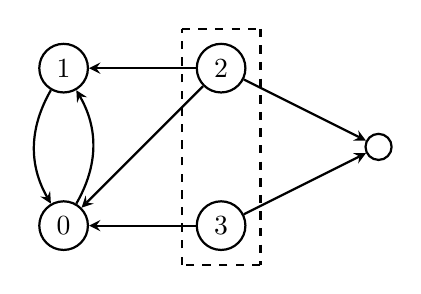
\begin{tikzpicture}
      [auto, thick,
  blk/.style={rectangle , draw=black , thick ,rounded corners,
  minimum height =2 em, align=center,text width=1.55cm, text=black,
   text opacity=1},
  nodeChain/.style={circle,draw=black, thick,minimum size=0.1cm,
  fill opacity=0.2,draw opacity=1, text=black,text opacity=1, align=center}
  ]
  \node[nodeChain] at (-2,-1) (zero) {0};
  \node[nodeChain] at (-2,1) (one) {1};
  \node[nodeChain] at (0,1) (two) {2};
  \node[nodeChain] at (0,-1) (three) {3};
  \node[nodeChain] at (2,0) (four){};
  \draw[-stealth] (zero) to[bend right]  (one);
  \draw[-stealth] (one) to[bend right]  (zero);
  \draw[-stealth] (two) -- (one);
  \draw[-stealth] (two) --  (zero);
  \draw[-stealth] (three) -- (zero);
  \draw[-stealth] (two) -- (four);
  \draw[-stealth] (three) -- (four);
  \draw[dashed] (-0.5,1.5) -- (0.5,1.5);
  \draw[dashed] (0.5,1.5)-- (0.5,-1.5);
  \draw[dashed]  (-0.5,-1.5) -- (-0.5,1.5);
  \draw[dashed]  (0.5,-1.5) -- (-0.5,-1.5);
\end{tikzpicture}
